\begin{figure}[htbp]
\centering
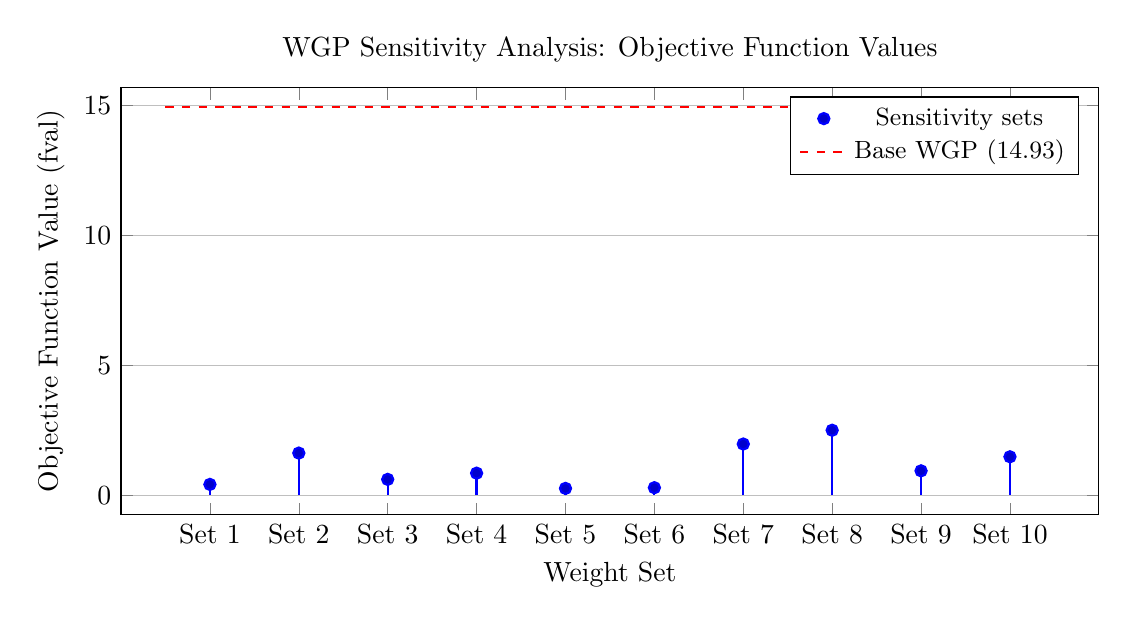
\begin{tikzpicture}
  \begin{axis}[
    title={WGP Sensitivity Analysis: Objective Function Values},
    xlabel={Weight Set},
    ylabel={Objective Function Value (fval)},
    xtick={1,2,3,4,5,6,7,8,9,10},
    xticklabels={Set 1, Set 2, Set 3, Set 4, Set 5, Set 6, Set 7, Set 8, Set 9, Set 10},
    width=14cm,
    height=7cm,
    ymajorgrids,
    ymin=0,
    enlargelimits=0.05,
    legend style={at={(0.98,0.98)},anchor=north east,font=\small},
  ]

  % Lollipop stems
  \addplot+[ycomb, mark=*, thick, blue] coordinates {
    (1,0.4128)
    (2,1.6183)
    (3,0.6062)
    (4,0.845)
    (5,0.2595)
    (6,0.286)
    (7,1.967)
    (8,2.4976)
    (9,0.935)
    (10,1.4761)
  };

  % Base WGP line
  \addplot[red, dashed, thick, domain=0.5:10.5] {14.9277};
  \addlegendentry{Sensitivity sets}
  
  \addlegendentry{Base WGP (14.93)}

  \end{axis}
\end{tikzpicture}
\caption{Lollipop plot of \textit{fval} across 10 weight sets (blue dots), compared with the base Weighted Goal Programming solution (red dashed line).}
\label{fig:wgp_sa_lollipop_fval}
\end{figure}
